\chapter{Rectangular Waveguide (3)}
%\begin{figure}
%\centering
%\includegraphics[width=1\linewidth]{\pathtoparttwo/graphics/Schematic-of-a-rectangular-waveguide-extending-along-z-a-and-the-TE10-top-and-TE11}
%\caption{}
%\label{fig:schematic-of-a-rectangular-waveguide-extending-along-z-a-and-the-te10-top-and-te11}
%\end{figure}
In the previous chapter, we tried to visualize the electric field inside a parallel plane waveguide. We also investigated the modal characteristics of a rectangular waveguide. We found that the mode that first propagates on a rectangular waveguide is a transverse electric mode with indexes (1, 0). We called that the \textbf{dominant mode of the rectangular waveguide}. 
	
We also argued that most of the time we went on to operate in this single mode or dominant mode on the waveguide to avoid dispersion i.e. broadening of the signal in the time domain and as it travels on a guided structure. So this TE$_{10}$  is the most important mode for a rectangular waveguide, because most of the time, the energy is going propagate in this mode. So when we conduct experiments in the laboratory or go to the fields, we mostly deal with the dominant mode,  TE$_{10}$ mode.
We also argued that most of the time we went on to operate in this single mode or dominant mode on the waveguide to avoid dispersion i.e. broadening of the signal in the time domain and as it travels on a guided structure. So this TE$_{10}$  is the most important mode for a rectangular waveguide, because most of the time, the energy is going propagate in this mode. So when we conduct experiments in the laboratory or go to the fields, we mostly deal with the dominant mode,  TE$_{10}$ mode.

In this chapter, we shall see the modal properties of the TE$_{10}$, mode and visualize the fields for TE$_{10}$ mode and then calculate the attenuation constant of a waveguide. This is because with practical waveguies there are two types of losses, losses in the walls and losses in the dielectric medium.

From Equations~\eqref{} \textemdash\;~\eqref{}, the varying fields in the TE mode are
\begin{align*}
E_{x} &= E_{z} = H_{y} = 0\\
E_{y} &= \frac{-j\omega\mu a }{\pi} C\sin(\frac{\pi x}{a}) e ^{-j\beta z}\\
H_{x} &= \frac{j\beta a}{\pi} C \sin(\frac{\pi x}{a})e^{-j\beta z} \\
H_{z} &= C\cos(\frac{\pi x}{a}) e^{-j\beta z}
\end{align*}
Again there is no y component for the magnetic field and ...
\begin{align}
\mathfrak{Re}\{E_{y}\} = A\sin(\frac{\pi x}{a})\sin(\frac{2\pi}{\lambda g}z)
\label{eqn:eyppw}\\
\mathfrak{Re}\{H_{x}\} = B\sin(\frac{\pi x}{a})\sin(\frac{2\pi}{\lambda g}z)\\
\mathfrak{Re}\{H_{z}\} = C\cos(\frac{\pi x}{a})\cos(\frac{2\pi}{\lambda g}z)
\end{align}

Considering the electric field, from Equation~\eqref{eqn:eyppw}, if $z = 0, E_{y}$ is zero. At a distance $ z = \frac{\lambda g}{4}$, $E_{y}$ is maximum for variation in z.

If we move the origin such that $z = \frac{\lambda g}{4}$ is now the starting point as shown in Figure~\ref{fig:lectureimage2}.
\begin{figure}[h]
\centering
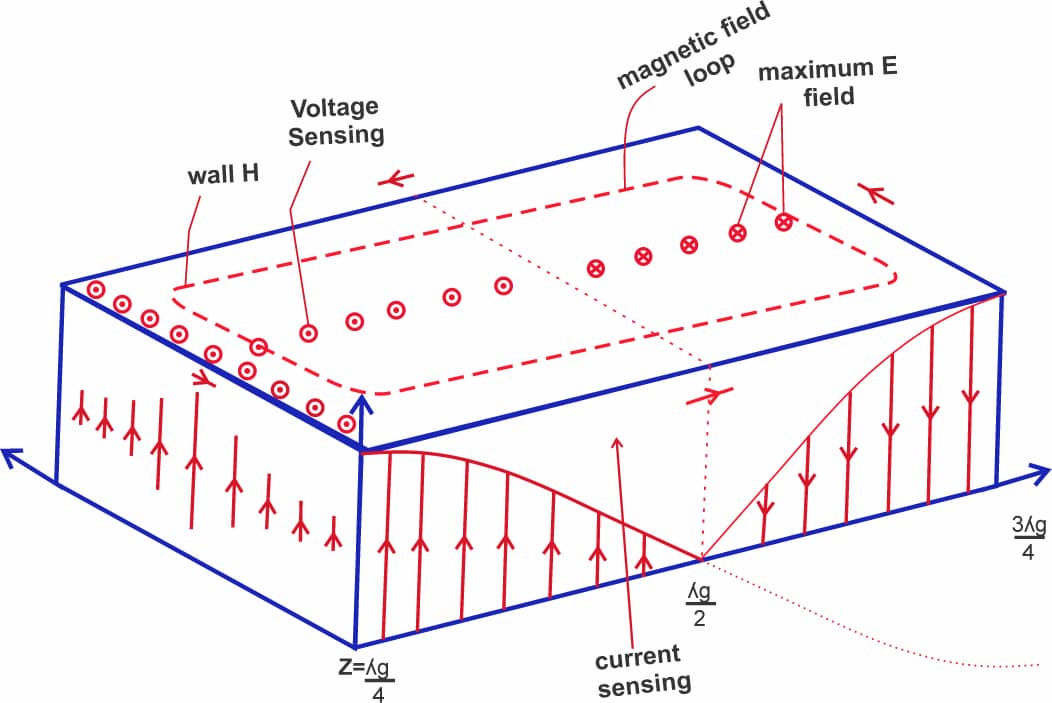
\includegraphics[width=1\linewidth]{\pathtoparttwo/graphics/lecture-image-2.jpg}
\caption{EM wave of a rectangular waveguide showing the field variations}
\label{fig:lectureimage2}
\end{figure}

$E_{y}$ will have a maximum value with sinusoidal variation along x as shown by the length of arrows and they all point in the positive y direction for $x = 0$ to $x = a$. Looking from the top, we have the variation shown with $\odot$ and $\otimes$ showing the direction of the field looking from the top. The size of the circles shows the strength of the field. So if we go sideways the field has a sinusoidal decrease, till it gets to zero at the edges.
 
So we can write down the plane and the side view for the waveguide. Visualizing the electric field is very simple as we visualize one component of the electric field, y oriented. The same thing can be done for magnetic fields.
\begin{figure}[h]
\centering
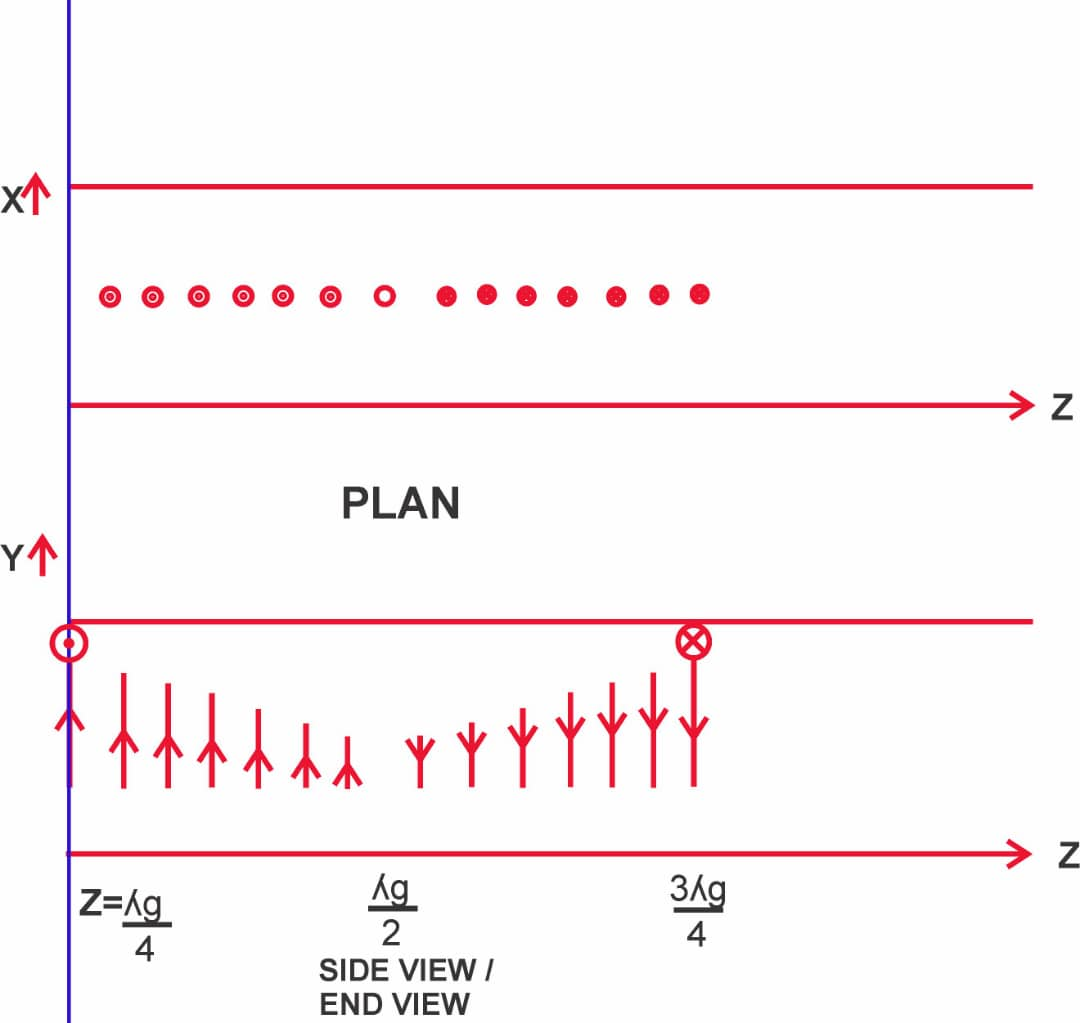
\includegraphics[width=1\linewidth]{\pathtoparttwo/graphics/lecture-image-3.jpg}
\caption{Plan and end view of an EM wave of a rectangular waveguide}
\label{fig:lectureimage3}
\end{figure}

As we have seen in the case of parallel plane waveguides, $H_{x}$ have variation the same as the electric field by $E_{y}$. $E_{y}$ and $H_{x}$ are maximum at the same point and minimum at the same point in space. But the z component of the magnetic field is shifted by $90^{o}$ or $\frac{\lambda g}{4}$ with respect to the x and z components. So wherever $H_{x}$ goes to zero, $H_{z}$ is maximum, so it is quadrature in x and z as we see in Figure~\ref{fig:lectureimage3}. We observe that;
\begin{align}
\mathfrak{Re}\{H_{x}\} = B\sin(\frac{\pi x}{a})\sin(\frac{2\pi}{\lambda g}z)\\
\mathfrak{Re}\{H_z\} = C\cos(\frac{\pi x}{a})\cos(\frac{2\pi}{\lambda g}z)
\end{align}

So where $H_{x}$ is maximum along z i.e  $z=\dfrac{\lambda g}{4}$, $H_{x}$ is minimum. The magnetic field lines are shown in Figure~\ref{fig:lectureimage3} with arrows designated 1, 2, 3 and 4\footnote{
Carefully observe $H_{x}$ and $H_{z}$ are maximum and where they occur.
}. So because the magnetic field must close on itself, 1, 2, 3, and 4 must form a loop as shown in Figure~\ref{fig:lectureimage2}. The variation of the magnetic field in the y-direction is zero. Hence $H_{x}$ and $H_{z}$ are constant in the y direction. So in the plan view, it appears as shown in Figure~\ref{fig:lectureimage2} with appropriate direction so that $E\times H$ gives the direction of propagation of the wave which is the z direction.

From the end view, at $z=\frac{\lambda g}{4}$ we have the magnetic field on the side wall coming out of the paper and at $z=\frac{\lambda g}{2}$, only $H_{z}$ is represented. At $z=\frac{3\lambda g}{4}$, we have $H_{x}$ going in the direction of $\otimes$. So if we visualize this field as a three-dimensional structure, the electric fields look like rods of various heights or various diameters, where diameters or the heights of the rod represent the strength of the electric field and the magnetic fields look like copies of rolled carpets or transformer stampings. Figure~\ref{fig:lectureimage4} shows a clearer visualization.
\begin{figure}[h]
\centering
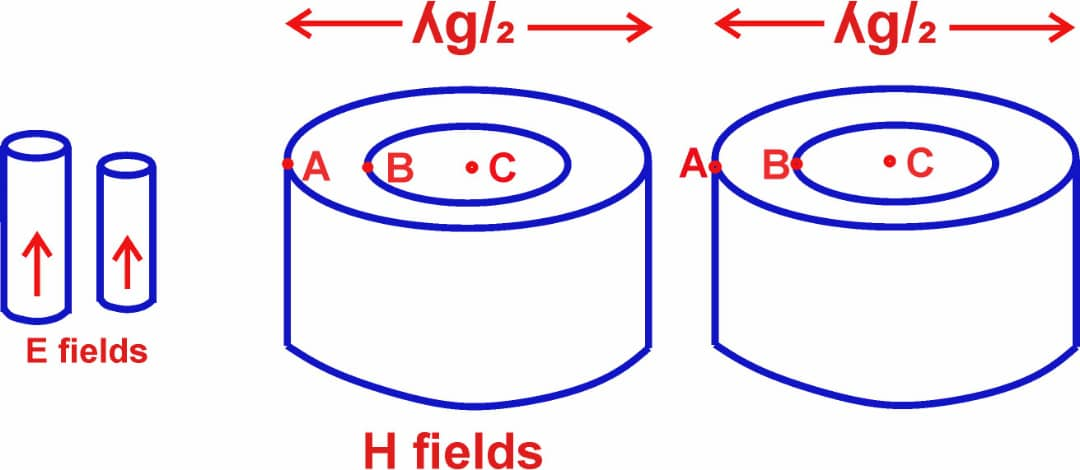
\includegraphics[width=1\linewidth]{\pathtoparttwo/graphics/lecture-image-4.jpg}
\caption{Representation of the field in three dimensions}
\label{fig:lectureimage4}
\end{figure}

Now that we get the field visualization at some instant of time, we say let this pattern move with the phase velocity inside the waveguide i.e the pattern starts drifting, so at every location, we sometimes see either A, B or C as shown in Figure~\ref{fig:lectureimage4}. Now we know that the electric field is maximum on the broader wall of the waveguide as mentioned earlier. For the TE$_{10}$ mode, the maximum electric field is along the broad wall along the plane $x = \frac{a}{2}$ as the wave travels in the z-direction. The magnetic field would be maximum on walls G and H. It does not vary with y so if we have to excite the waveguide by electric fields, with a voltage probe, then the probe must be placed on the line of the broader wall (ie $x = \frac{a}{2}$ middle point) so that the electric field is excited and that electric field gives excitation corresponding to TE$_{10}$. However, if we have a current probe, we put it on the side walls of G and H which can excite the field distributions we have visualized. Then this would help in exciting TE$_{10}$ mode inside the waveguide. The same thing is true if the waveguide has some modal properties and we want to sense the voltage and current on this waveguide, the voltage probe must be mounted on the broader wall and the current probe must be mounted on the sidewall G and H. This is the way the fields inside a rectangular waveguide are detected by using the voltage and current probe, or excited by giving signals to the probe protruding into the waveguides and then exciting a field inside a structure.

So this visualization of the field for the dominant mode which is th the TE$_{10}$ mode is quite useful because it also tells us how the excitation of the field can be achieved by putting voltage and current probes on the wall of the waveguides. Having understood the field distribution in the  TE$_{10}$ mode with an electric field more like a rod and a magnetic field more like rolled carpet or transformer stamping, we can very easily draw the electric and magnetic field for higher order modes. Let us say we want to excite the TE$_{20}$ mode for the rectangular waveguide.
So this visualization of the field for the dominant mode which is th the TE$_{10}$ mode is quite useful because it also tells us how the excitation of the field can be achieved by putting voltage and current probes on the wall of the waveguides. Having understood the field distribution in the  TE$_{10}$ mode with an electric field more like a rod and a magnetic field more like rolled carpet or transformer stamping, we can very easily draw the electric and magnetic field for higher order modes. Let us say we want to excite the TE$_{20}$ mode for the rectangular waveguide.

Of course, we can write down the field expressions for electric and magnetic fields. Then, do the same thing we did for TE$_{10}$ and visualize the fields. However, once we understand that electric and magnetic fields are in a specific form, we can stretch our imagination a bit to visualize electric and magnetic fields for this higher-order mode.
Of course, we can write down the field expressions for electric and magnetic fields. Then, do the same thing we did for TE$_{10}$ and visualize the fields. However, once we understand that electric and magnetic fields are in a specific form, we can stretch our imagination a bit to visualize electric and magnetic fields for this higher-order mode.

The index 2 in TE$_{20}$ mode represents that there are two cycles in the x direction and no variation in the y direction. So the electric field always lies in the y direction. Regarding the magnetic fields, they are like transformer stampings or rolled carpets and we have two sections each would have a magnetic loop shown in Figure~\ref{fig:lectureimage4}. The direction of the magnetic field will be such that the Poynting vector is in the z-direction. All the fields are essentially going together in the region between the two magnetic loops, so we have two rolled carpets stacked against each other in the waveguide of TE$_{20}$ mode. So once a basic understanding of visualizing fields is developed, it is easy to visualize the fields for higher-order modes.

\section{Surface Current on a rectangular waveguide}\index{surface current}
The next question we ask is when the fields are excited inside this waveguide, will surface current be induced in the waveguide? Again we come back to TE$_{10}$ mode. We have seen that surface current is related to the tangential component of magnetic fields. So in the figure above, on the top and bottom walls, the direction of the magnetic field keeps changing, however on the side walls, the direction of the magnetic field is always along the z-direction. Though magnitude is changing, it is always along the z direction. So $\hat{n} \times H$ of side walls is in the negative y direction.
The next question we ask is when the fields are excited inside this waveguide, will surface current be induced in the waveguide? Again we come back to TE$_{10}$ mode. We have seen that surface current is related to the tangential component of magnetic fields. So in the figure above, on the top wall, the direction of the magnetic field keeps changing, however on the side walls, the direction of the magnetic field is always along the z-direction. Though magnitude is changing, it is always along the z direction. $\hat{n} \times H$ of side walls, $H$ is in the negative y direction.
\begin{figure}[h]
\centering
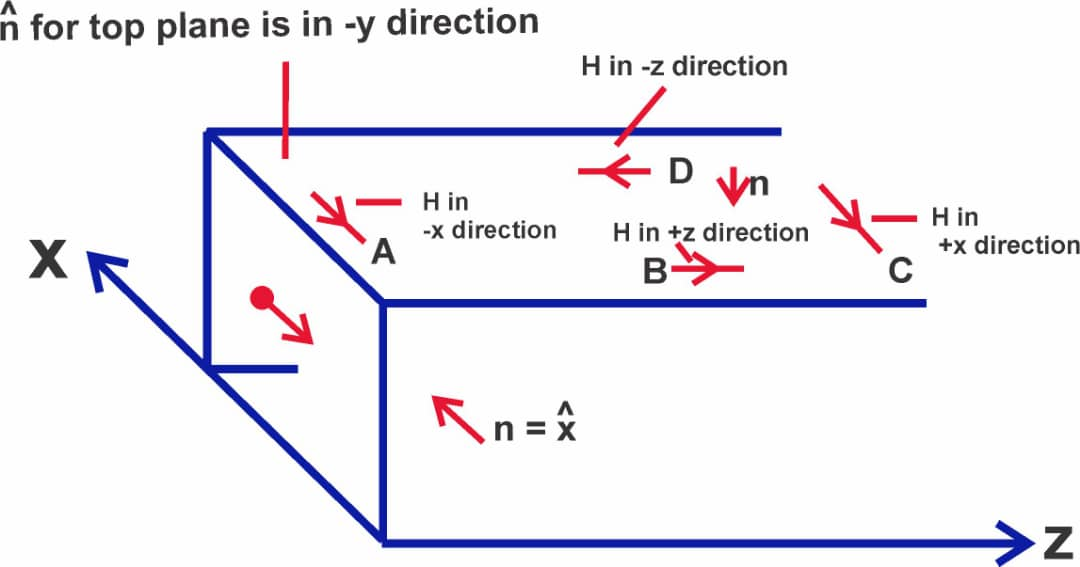
\includegraphics[width=1\linewidth]{\pathtoparttwo/graphics/lecture-image-5.jpg}
\caption{Direction of the surface current and magnetic field in a rectangular waveguide}
\label{fig:lectureimage5}
\end{figure}
\begin{figure}[h]
\centering
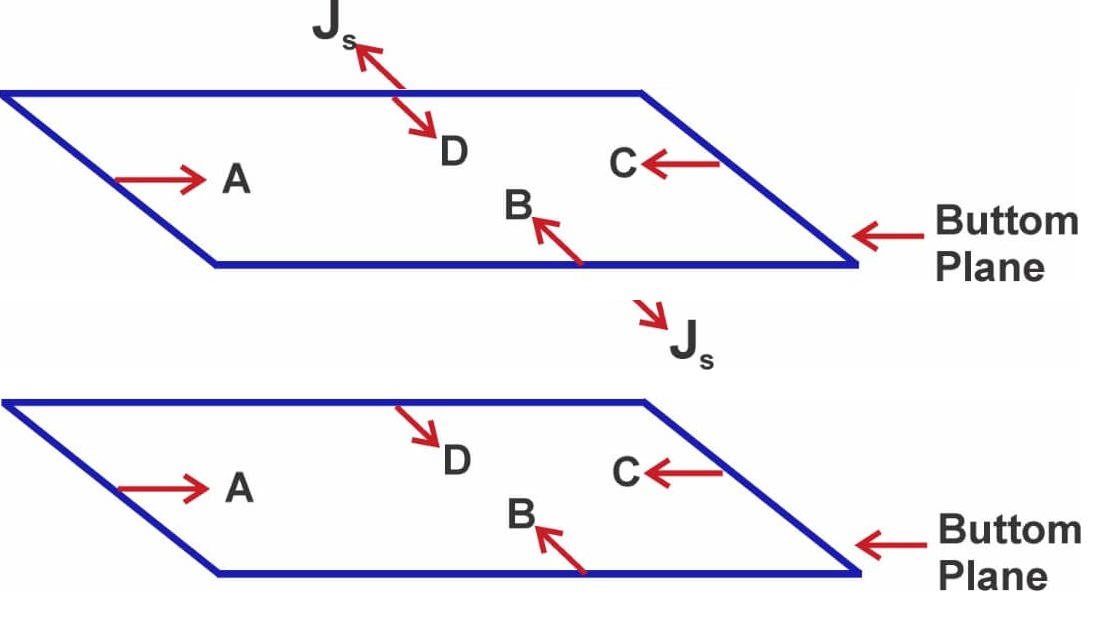
\includegraphics[width=1\linewidth]{\pathtoparttwo/graphics/lecture-image-6.jpg}
\caption{Direction of the surface current and magnetic field on the top and bottom walls of a rectangular waveguide}
\label{fig:lectureimage6}
\end{figure}

On the top plane, At
\begin{align*}
\hat{n} \times H &= -\hat{y} \times (-\hat{x})= -\hat{z}\\
\hat{n} \times H &= -\hat{y} \times (+\hat{z})= -\hat{x}\\
\hat{n} \times H &= -\hat{y} \times (+\hat{x})= \hat{z}\\
\hat{n} \times H &= -\hat{y} \times (-\hat{z})= \hat{z}
\end{align*}
Hence we see the variation of $J_{s}$ as it keeps changing direction in the plane.

For the right side wall, it is in the z direction ($+z$) and for the left side wall, it is in the negative z direction. The left side wall   
\begin{equation}
n\times H = -\hat{x} \times (-\hat{z})= -\hat{y}
\label{eqn:negy}
\end{equation}
The right side wall 
\begin{equation}
n \times H = \hat{x} \times (\hat{z}) = \hat{y}
\label{eqn:posy}
\end{equation}
From these equations, the surface current is going in the y-direction only upon one face down and the other sign is immaterial here.
	
The bottom plane has the opposite direction for $J_{s}$ corresponding to the top plane as calculated and it is shown above. So looking at the current distribution for all four walls and combining them together, we have the Figure~\ref{fig:lectureimage10}. Considering the right wall, the magnetic field is in the z-direction and at $\pi$ region (see Figure~\ref{fig:surface_current_te10}), $J_{s}$ is in the y-direction as we have solved in Equations~\ref{eqn:negy} and \ref{eqn:posy}. On the top wall, the normal direction is y, so then we have a situation shown where it is as if the current is just coming out of the top plane or coming into a point on the top plane or bottom plane depending on the location under consideration. 
\begin{figure}[h]
\centering
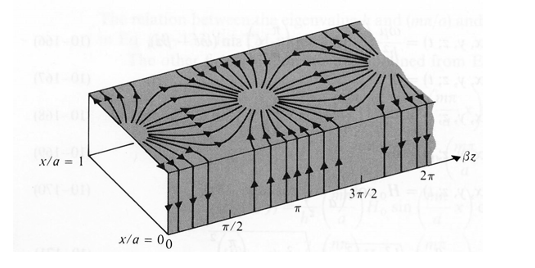
\includegraphics[width=1\linewidth]{\pathtoparttwo/graphics/surface_current_te10.png}
\caption{Surface current distribution on a rectangular waveguide}
\label{fig:surface_current_te10}
\end{figure}

So on the side wall, the current does not change as $H$ on the side wall was also constant. It is zero at the centre of the top plane, it increases as we get to the side of the top plane, remains constant on the side wall, and then decreases till it becomes zero on opposite points to the top wall where $H$ started from. In fact, the current is as if it is starting from nowhere it grows and dies down on the opposite wall where at the location it started. In the next half cycle, the direction of the current will change and this repeats itself periodically. In a half cycle, the current flows upward that is the charge moves downward. In another half cycle, the current flows downward i.e. the electrons move upward. So the accumulation of charges takes place between two walls and the charges keep going back and forth and essentially the current flows on the surface of the waveguide. So for every $\frac{\lambda g}{2}$ we have a current island created. It grows and becomes maximum and then decreases to zero on the top plane and bottom plane. It repeats this every $\frac{\lambda g}{2}$. So the current flow is like a blooming flower around both sides, with one like a source and another like a sink of current on the opposite top and bottom plane.
	
So this is how the current is going to get induced on the rectangular waveguide. This current helps us to also find out if we cut the waveguide and allow some slots inside the waveguide, we will see later in antennas that if the current is disrupted, then there is a possibility of getting radiation from the system. So if the current direction in the waveguide is known. Then we know where we should cut the slots in the waveguide. So that there is a possibility of radiation. If we cut a slot that does not distort the current flows, as shown in Figure~\ref{fig:lectureimage10}.
\begin{figure}[h]
\centering
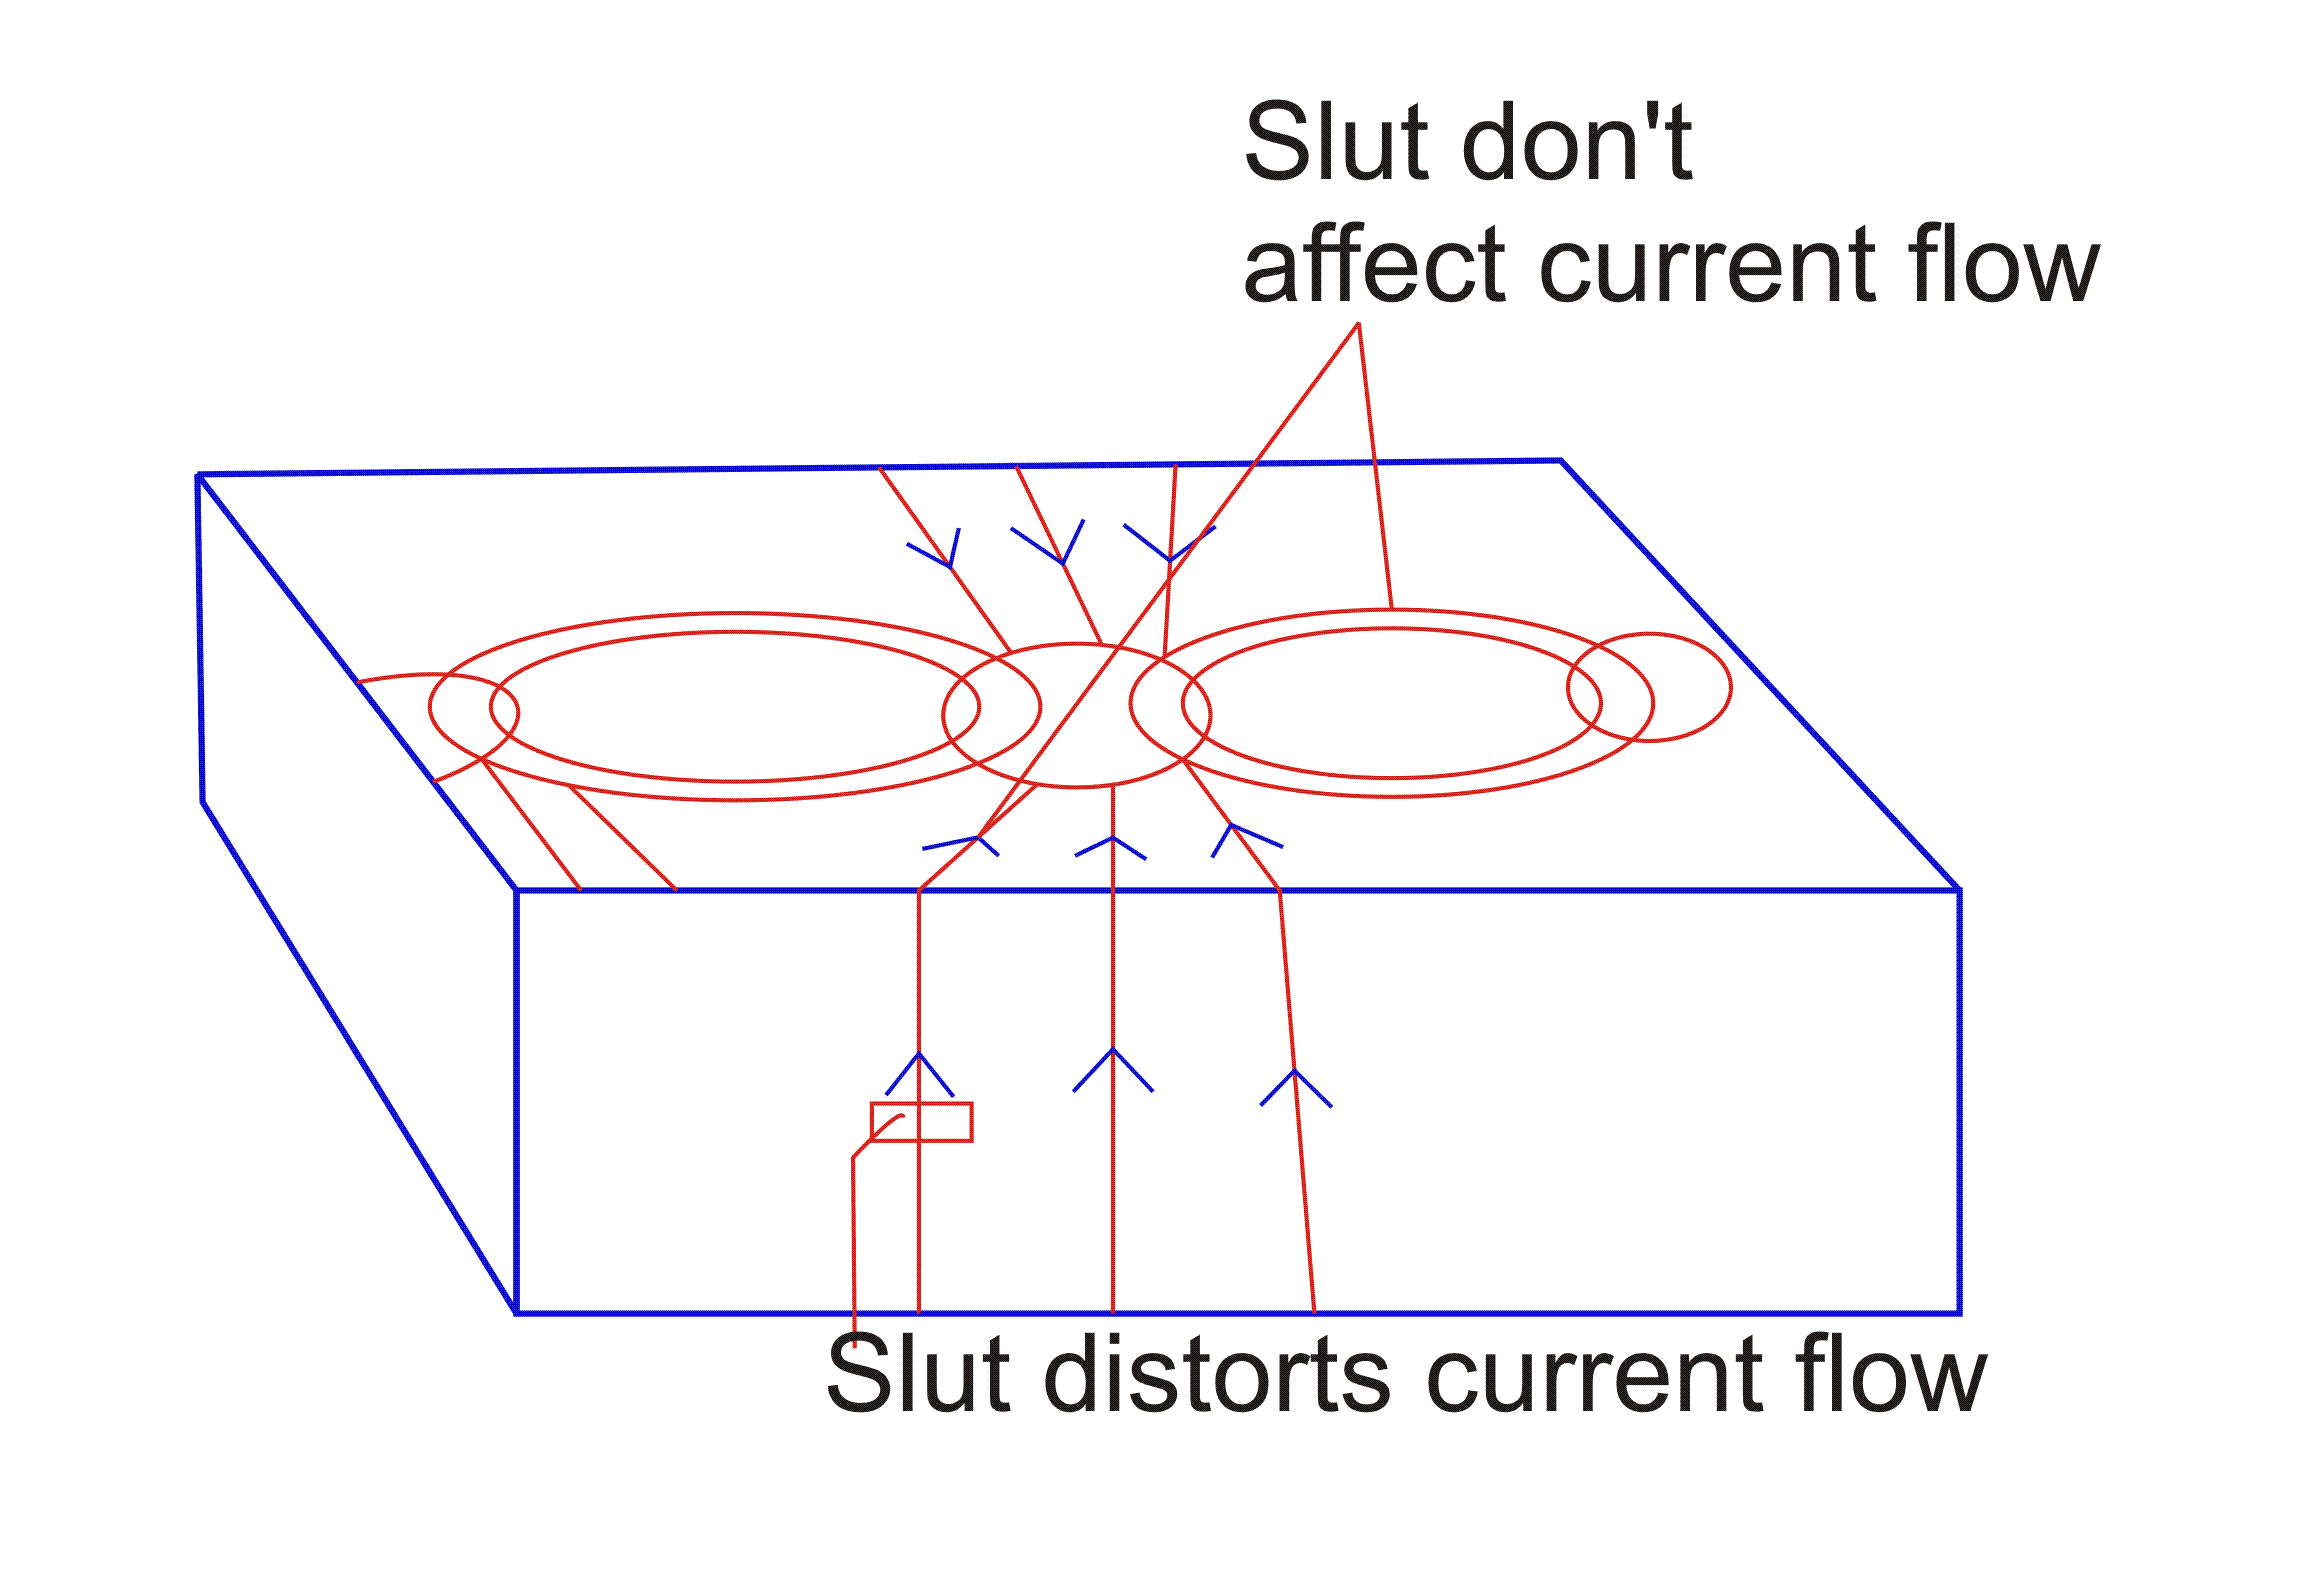
\includegraphics[width=1\linewidth]{\pathtoparttwo/graphics/lecture-image-10.png}
\caption{Diagram showing the relationship between slot openings and current flow}
\label{fig:lectureimage10}
\end{figure}

Thus, there is a higher possibility of radiation if we know the current direction flow on the waveguide and we know where to cut the slots on the waveguide to get radiation. Another usefulness of finding current direction is if the walls are not ideal conductors, the current flowing will create ohmic losses, which means the power should have been propagated inside the waveguide, part of it will get lost in ohmic heating of the waveguides and this is related to the current distribution on the walls. So the knowledge of current distribution is useful in finding out how the structure can be made to radiate and also how the losses will change if the walls are not ideal conductors.
	
With this, we can go to the next important topic in waveguides i.e the loss calculation in the rectangular waveguide. We have seen that if the structure is not ideal i.e the dielectric filling the waveguide is not an ideal dielectric, and if the conductor is not ideal conductor, i.e conductivity is not infinite there will always be loss of energy when it propagates through the structure.

\section{Attenuation Constant}
Now we try to find out what is the loss per unit length of a rectangular waveguide. As we know, it is measured by a parameter called \textbf{attenuation constant}\index{attenuation constant}. We have seen this parameter in the transmission line, that if there is a loss in the transmission line, the variation will be $e^{-\alpha z}$ where $\alpha$ is the attenuation constant. So all the fields exponentially decay as we travel along the structure. 

Here we assume that the attenuation constant will cause exponential decay of the fields as they travel. We are interested in finding out the attenuation constant of the conductivity parameter for the walls and the loss in the dielectric if given. However, the problem, in this case, is a little complicated and for this simple reason, if we consider an arbitrary loss in the wall, and arbitrary loss in the dielectric, the modal analysis which we have carried out has to be modified. This is because of the field distribution we earlier assumed which had ideal conductors and ideal dielectric. So in the presence of loss, the electric and magnetic fields are going to get modified, and modification of electric and magnetic fields will change the loss since the loss is related to current distribution. So essentially we are in a loop that the loss calculation requires the knowledge of electric and magnetic fields and the electric and magnetic fields depend on the loss.
	
The problem is very complicated, in fact, if we went to solve this for an arbitrary loss, in the dielectric for arbitrary conductivity of the walls, if we assume that the primary function of this waveguide was to transfer energy from one point to the other efficiently, we make every effort to get the losses as minimum as possible. That means we make a waveguide of a material which has as high conductivity as possible and fill this waveguide with a dielectric as pure as possible. So normally the loss which takes place either in the dielectric filling this waveguide or the finite conductivity of the conducting plane is very very small. Under the assumption, then we can say that as a first order, the fields do not get disturbed significantly because of the losses in the waveguide. What this means is we assume that the fields we got for any of the modes are exactly the same as the lossless waveguides even in the presence of this small loss. So we said that we have a full knowledge of the electric and magnetic fields and once we say that, the loop is broken. So from the knowledge of electric and magnetic fields, we can find out what is the current, from there we can find out what is the ohmic losses and then we can calculate the attenuation constant. Normally what we will do since the attenuation is consisting of two components viz, loss in the dielectric and then the loss in the conducting walls, is that we separate out these two losses. We say well since the losses are very small, when we calculate dielectric losses, we assume that the waveguide is made of high conductance. When we calculate the conductive losses we assume the waveguide is filled with ideal dielectric. So if we say we have attenuation constant $\alpha$, it consists of two components and two first-order approximations, $\alpha$ is the sum of two alphas, $\alpha_{d}$ for dielectric loss and  $\alpha_{c}$ for conductor loss. So $\alpha =  \alpha_{d} +  \alpha_{c}$. When calculating $\alpha_{c}$ we assume  $\alpha_{d} = 0$ and when calculating  $\alpha_{d}$, we assume  $\alpha_{c} = 0$.
	
\subsection{Dielectric Attenuation constant}
In calculating  $\alpha_{d}$ we use the same approach we used for a transmission line. That is we calculate the propagation constant $\beta$ and from the dispersion relation, simply replace the dielectric constant with the dielectric constant of a lossy medium. From Equation~\eqref{}, considering a rectangular waveguide in TE$_{10}$ mode, we have
\begin{equation}
\footnotemark\beta_l^{2} = \omega^{2}\mu\epsilon_{l} -\left(\frac{\pi}{a}\right)^{2}
\label{eqn:dispersrelte10}
\end{equation}
\footnotetext{
We rewrite $\beta$ as $\beta_l$ to indicate that the propagation constant is for a lossy medium.
}
$\epsilon_{l}$ is the relative permittivity for lossy medium given as:
\begin{align*}
\epsilon_{l} = \epsilon_{o}\epsilon_{rl}
\end{align*}
But $\epsilon_{rl} = \epsilon_{r}(1-j\tan\delta)$ and $\tan\delta$ is the loss tangent. We substitute for $\epsilon_{l}$ in Equation~\eqref{eqn:dispersrelte10} so that
\begin{equation*}
\beta^{2}_{l} = \omega^{2}\mu\epsilon_{o}\epsilon_{r}(1-j\tan\delta)
\end{equation*}
\begin{dmath*}
\beta^{2}_{l} = \omega^{2}\mu\epsilon_{o}\epsilon_{r} - j\omega^{2}\mu\epsilon_{o}\epsilon_{r}\tan\delta
= \beta^{2} - j\beta^{2}\tan\delta\quad\text{since $\beta$ for lossless medium is $\omega\sqrt{\mu\epsilon}$}
\end{dmath*}
\begin{dmath}
\beta_{l} = (\beta^{2} - j\beta^{2}\footnotemark\tan\delta)^{\frac{1}{2}}
\simeq \beta - \frac{j\beta\tan\delta}{2}
\end{dmath}
\footnotetext{
$\tan\delta$ is usually small for a low-loss dielectric medium.
}
So we have a phase constant $\beta_{l}$ which has a real and imaginary part. The real part is $\beta$ whereas the imaginary part is the attenuation constant due to lossy dielectric filling the waveguide.

\begin{align}
\alpha_{d} = \frac{\beta\tan\delta}{2}
\label{eqn:alphad}
\end{align}
Recall in waveguide the variation along z is $e^{-j\beta z}$ so you need imaginary values of $\beta$ to give you attenuation. A real value would give oscillatory terms in $\cos\beta z$ and $\sin\beta z$ while an imaginary term such as $\alpha_d$ yeilds $e^{-j}(\frac{j\beta\tan\delta}{2})$, an exponentially decaying term.

We can simplify $\alpha_d$ further since we know that $\tan\delta = \frac{\sigma}{\omega\epsilon_{o}\epsilon_{r}}$, We substitute into Equation~\eqref{eqn:alphad} to get
\begin{dmath}
\alpha_{d} = \frac{\beta \frac{\sigma}{\omega\epsilon_\circ\epsilon_r}}{2}
= \frac{\beta^2 \frac{\sigma}{\omega\epsilon_\circ\epsilon_r}}{2\beta}
= \frac{\omega^2\mu\epsilon_\circ\epsilon_r\sigma}{2\beta\omega\epsilon_\circ\epsilon_r}
= \frac{\omega\mu\sigma}{2\beta}
\label{eqn:attenuationconst}
\end{dmath}
We can express $\alpha_d$ in terms of the cut-off frequency by considering the propagation constant of a lossless medium, $\beta$.

For lossless cases, 
\begin{equation*}
\beta = \sqrt{\omega^{2}\mu\epsilon-\left(\frac{m\pi}{a}\right)^{2}-\left(\frac{n\pi}{b}\right)^{2}}
\end{equation*}
But for TE$_{10}$ we have that cutoff frequency, $\beta = 0$, that is
\begin{equation*}
\omega^{2}_{c}\mu\epsilon = \left(\frac{m\pi}{a}\right)^{2}+\left(\frac{n\pi}{b}\right)^{2}
\end{equation*}
As such
\begin{dmath*}
\beta = \sqrt{\omega^{2}\mu\epsilon-\omega^{2}_{c}\mu\epsilon} = \omega\sqrt{\mu\epsilon}\sqrt{1-\left(\frac{fc}{f}\right)^{2}}
\end{dmath*}
Substituting for $\beta$ in the Equation~\ref{eqn:attenuationconst}
\begin{dmath*}	
\alpha_{d}=\frac{\omega\mu\sigma}{2\beta}= \frac{\omega\mu\sigma}{2\omega\sqrt{\mu\epsilon}\sqrt{1-\left(\frac{fc}{f}\right)^{2}}}
\end{dmath*}
Dividing the numerator and denominator by $\omega\sqrt{\mu\epsilon}$
\begin{dmath}
\alpha_{d} = \frac{\sigma\sqrt{\frac{\mu}{\epsilon}}}{2\sqrt{1-\left(\frac{fc}{f}\right)^{2}}}=\frac{\sigma\eta}{2\sqrt{1 - \left(\frac{fc}{f}\right)^{2}}}
\label{eqn:attenuationconst2}
\end{dmath}
where $\eta= \sqrt{\frac{\mu}{\epsilon}}$. Therefore Equation~\ref{eqn:attenuationconst2} is the formula for the attenuation constant and $f_c$ is the cut-off frequency of the mode under consideration.

So knowing the dielectric constant of the medium and assuming the loss tangent is very small, ie the losses in the medium are very small, we can establish the attenuation constant $\alpha_{d}$ due to the finite conductivity of the dielectric medium. We say that for two losses, the attenuation constant is proportional to the conductivity of the medium and we see that $\alpha_{d}$ is related to the cut-off frequency. So when the frequency is much larger compared to $f_{c}$, we have $\frac{\sigma\eta}{2}$ which is very similar to the case of the transmission line. We recall that if we take the transverse electromagnetic mode, $\frac{\sigma\eta}{2}$ was the attenuation constant for the transmission line.

So when we talk about the lossy mediums in the unbound medium, earlier we got a loss which was $\alpha = \frac{\sigma\eta}{2}$. What happens now however is that in the rectangular waveguide, it also depends upon how far away you are from the cut-off frequency, so if you are very close to the cut-off frequency, $\sqrt{1 - \left(\frac{fc}{f}\right)^{2}}$ becomes close to zero and Equation~\eqref{eqn:attenuationconst2} becomes very large. So now the dielectric loss is a function of frequency which otherwise was not a function of frequency. In the transverse electromagnetic mode,  $\alpha_{d}$ only depended on the conductivity. So $\alpha_{d}$ is proportional to the conductivity of the dielectric $\sigma$ and also depends on how far away you are from the cut-off frequency of a particular mode. As you get closer to the mode's cut-off frequency, your dielectric loss increases, so by using the equation, we can calculate one component of the attenuation constant and that is the dielectric attenuation constant $\alpha_{d}$.

\subsection{Conductor Attenuation constant}
The second component we want to calculate now is the finite conductivity of the boundary. This calculation is not as straightforward as the dielectric attenuation constant we have just done. Since the fields are now inside the waveguide, simply modifying the propagation constant would do, but we do not know now how to put this medium as a lossy medium. If the losses are going to take place in the walls, then we have to go from the first principle and calculate the attenuation constant using the first principles. What this means is that if there is a loss in the medium, the $E$ and $H$ fields vary as a function of $z$ ie $ {\hat{E}}, {\hat{H}} \ \sim\ e^{-\alpha z}$ where $\alpha$ is the attenuation constant. So the power which is proportional to $|{\hat{E}}|^{2}$ or $|{\hat{H}}|^{2}$ since power is ${\hat{E}}\times{\hat{H}}$. So power density is the power which the waveguide carriers, i.e. $W\sim e^{-2\alpha z}$ ie varies as $e^{-2\alpha z}$. We can differentiate power, $W$, with respect to z to get 
\begin{dmath*}
\dv{W}{z}\sim-2\alpha e^{-2\alpha z} = -2\alpha W 
\end{dmath*}
So $\alpha$ is the attenuation constant in general and can be expressed as
\begin{equation*}
\alpha = \frac{\dv{W}{z}}{2W}
\label{eqn:calcalpha}
\end{equation*}

Physically -$\dv{W}{z}$ stands for the rate at which power decrease in the direction $z$ or in the direction of the wave propagation, and $W$ is the total power carried by the structure. Now that the attenuation constant can be calculated by two quantities i.e. power loss per unit length $(-\dv{W}{z})$  along the waveguide, divided by two times the power carried by the waveguide. This can be represented in general as
\begin{dmath}
\alpha = \frac{\textnormal{Power decrease / unit length}}{2\times \textnormal{Total power carried by the waveguide}}
\end{dmath}

Now to calculate the attenuation constant, we require two quantities to be calculated viz power loss per unit length and the total power carried by the waveguide. Thus, we have to calculate the rate of power loss and power carried which requires the knowledge of the $E$ and $H$ fields in the waveguide and surface current in its walls. So surface current will give us the loss, and we can calculate it per unit length i.e. what is the power loss in the waveguide? Calculating $E\times H$ will give the Poynting vector and integrating over the cross-sectional area of the waveguide gives the total power flowing inside the waveguide. 

So $W = \int\frac{1}{2}\mathfrak{Re}\{\bar{E}\times\bar{H^*}\}\cdot{da}$ gives the total power flowing in  the waveguide. Once we know the surface current $J_{s}$ on these walls, then we see that power loss per unit area is given by half surface resistance, $R_s$, multiplied by $|J_{s}|^{2}$. So knowing the surface current, we can calculate the loss per unit area and since the height of the waveguide is known, we can calculate the loss per unit length of the waveguide. Once we know these two quantities, using Equation~\eqref{eqn:calcalpha}, we can calculate the attenuation constant of this waveguide due to the finite conductivity of the walls.

In the next chapter, by using this basic definition of the attenuation constant, we will derive the attenuation constant for two modes. One mode is for a parallel plane waveguide in the TEM mode, i.e the simplest mode just to get a feel of how to calculate this quantity. Then we would calculate the attenuation constant for a rectangular waveguide for TE$_{10}$ mode.

\section*{Exercises}
\begin{ExerciseList}
\Exercise[label={ex411}]
What is the dominant mode in a rectangular waveguide, and why is it important?

\Exercise[label={ex412}]
How are the electric and magnetic fields visualized inside a parallel plane waveguide? And what are the field patterns for TE$_{10}$ mode in a rectangular waveguide?

\Exercise[label={ex413}]
What is the attenuation constant in a waveguide, and how is it related to loss in waveguides? How is the attenuation constant affected by dielectric losses and conductor losses? And how does the loss tangent affect the attenuation constant in dielectric-filled waveguides?

\Exercise[label={ex414}]
How is surface current induced in a rectangular waveguide? And what is the relationship between surface current and magnetic field direction on different walls of the waveguide?

\Exercise[label={ex415}]
How is the attenuation constant related to power loss and total power carried by the waveguide?
\end{ExerciseList}
